\documentclass[11pt]{article}

\usepackage{physics}
\usepackage[top=1in, bottom=1in, left=0.5in, right=0.5in]{geometry}
\usepackage{hanging}
\usepackage{amsfonts, amsmath, amssymb}
\usepackage[none]{hyphenat}
\usepackage{fancyhdr}
\usepackage[nottoc, notlot, notlof]{tocbibind}
\usepackage{graphicx}
\graphicspath{{./images/}}
\usepackage{float}
\usepackage{siunitx}
\usepackage{esint}

\pagestyle{fancy}
\fancyhead{}
\fancyfoot{}
\fancyhead[L]{MAP2302 Professor Jury}
\fancyhead[R]{Sai Sivakumar 10/14/20}
\fancyfoot[R]{\thepage}
\renewcommand{\headrulewidth}{0pt}

\setlength{\parindent}{0cm}
\setlength{\parskip}{5pt}
\renewcommand{\baselinestretch}{1.25}

\newcommand{\ihat}{\boldsymbol{\hat{\textbf{\i}}}}
\newcommand{\jhat}{\boldsymbol{\hat{\textbf{\j}}}}
\newcommand{\dr}{\vec{r}~^{\prime}(t)}
\newcommand{\dx}{x^{\prime}(t)}
\newcommand{\dy}{y^{\prime}(t)}

\newcommand{\br}[1]{\left(#1\right)}
\newcommand{\sbr}[1]{\left[#1\right]}
\newcommand{\cbr}[1]{\{#1\}}

\newcommand{\dprime}{\prime\prime}

\usepackage{mathtools}

\DeclarePairedDelimiterX{\abr}[1]{\langle}{\rangle}{#1}

\setcounter{page}{1}

\begin{document}
Section 4.2 Problems 9, 15, 46, Section 4.3 Problems 7, 21, 35, and Section 5.4 Problems 1, 11\\

Section 4.2 \\

9. $4y^{\dprime}-4y^{\prime}+y = 0$ Solve.

Use differential operators to write the differential equation as:
$$\br{D^2-D+
\frac{1}{4}}y = 0 \to \br{D-\frac{1}{2}}\br{D-\frac{1}{2}}y = 0$$

Let $u = \br{D-\frac{1}{2}}y$ and we solve the following equation:
$$\br{D-\frac{1}{2}}u = 0 \to \dv{u}{t} = \frac{1}{2}u \to u = e^{\frac{1}{2}t}$$

Then
$$\br{D-\frac{1}{2}}y = e^{\frac{1}{2}t} \to \dv{y}{t} - \frac{1}{2}y = e^{\frac{1}{2}t} \to \int 1 \dd{\br{e^{-\frac{1}{2}t}y}} = \int 1 \dd{t} \to y = te^{\frac{1}{2}t}$$

Hence the solution curve is of the form:
$$y = C_1e^{\frac{1}{2}t} + C_2te^{\frac{1}{2}t}$$ \\

15. $y^{\dprime} -4y^{\prime} + 3y = 0$; $y(0) = 1$, $y^{\prime}(0) = \frac{1}{3}$ Solve.

Use differential operators to write the differential equation as:
$$\br{D-1}\br{D-3}y = 0$$

We know the general solution to a differential equation of this form, and for this specific one it is:
$$y = C_1e^t+C_2e^{3t}$$

Differentiate once and use the initial value $y^{\prime}(0) = \frac{1}{3}$ and then use the other initial value $y(0) = 1$:
$$C_1 + 3C_2 = \frac{1}{3}$$
$$C_1 + C_2 = 1$$

Evidently $C_2 = -\frac{1}{3}$ and $C_1 = \frac{4}{3}$, so the solution curve solving the IVP is of the form:
$$y = \frac{4}{3}1e^t-\frac{1}{3}e^{3t}$$ \\

46.

(a) Rewrite the differential equation $y^{\dprime} - y = 0$ using differential operators:
$$\br{D^2-1}y = 0 \to \br{D-1}\br{D+1}y = 0$$

Using what we know about differential equations of this form we can say that the general solution is given by:
$$y = C_1e^t + C_2e^{-t}$$

For $\cosh(t)$ we have the following system of equations given by the initial values $y^{\prime}(0) = 0$, $y(0) = 1$:
$$C_1 - C_2 = 0$$
$$C_1 + C_2 = 1$$

Evidently $C_1 = C_2 = \frac{1}{2}$, so we have:
$$\cosh(t) = \frac{e^t + e^{-t}}{2}$$

For $\sinh(t)$ we have the following system of equations given by the initial values $y^{\prime}(0) = 1$, $y(0) = 0$:
$$C_1 - C_2 = 1$$
$$C_1 + C_2 = 0$$

Evidently $C_1 = \frac{1}{2}$ and $C_2 = -\frac{1}{2}$, so we have:
$$\sinh(t) = \frac{e^t - e^{-t}}{2}$$

Then since we know that $\dv{t}e^{-t} = -e^{-t}$ it follows that $\dv{t}\cosh(t) = \sinh(t)$ and $\dv{t}\sinh(t) = \cosh(t)$:
$$\dv{t}\frac{e^t + e^{-t}}{2} = \frac{e^t - e^{-t}}{2} \text{ and } \dv{t}\frac{e^t - e^{-t}}{2} = \frac{e^t + e^{-t}}{2}$$ \\

(b) Write in the explicit definition of the hyperbolic sine and cosine for $y = c_1\cosh(t) + c_2\sinh(t)$:
$$y = c_1\frac{e^t + e^{-t}}{2} + c_2\frac{e^t - e^{-t}}{2}$$

Absorbing the division by 2 into the constants $c_1$ and $c_2$, and using some algebra we find that the solution curve 
$$y = \br{c_1+c_2}e^t + \br{c_1-c_2}e^{-t}$$

is of the form we deduced above and thus solves the differential equation $y^{\dprime} - y = 0$. \\

(c) Since we can rewrite (using differential operators) $ay^{\dprime} + by^{\prime} + cy = 0$ as $\br{D-\br{\alpha - \beta}}\br{D-\br{\alpha + \beta}}y = 0$ we can give a general solution to the differential equation as:
$$y = c_1e^{\br{\alpha - \beta}t} + c_2e^{\br{\alpha + \beta}t}$$

Give another solution as $y = -c_2e^{\br{\alpha - \beta}t} + c_1e^{\br{\alpha + \beta}t}$ and add both solutions together to form:
$$y = c_1e^{\br{\alpha - \beta}t} + c_2e^{\br{\alpha + \beta}t} - c_2e^{\br{\alpha - \beta}t} + c_1e^{\br{\alpha + \beta}t}$$

Then some algebra:
$$y = c_1e^{\alpha t}e^{-\beta t} + c_2e^{\alpha t}e^{\beta t} - c_2e^{\alpha t}e^{-\beta t} + c_1e^{\alpha t}e^{\beta t} \to 2c_1e^{\alpha t}\br{\frac{e^{\beta t} + e^{-\beta t}}{2}} + 2c_2e^{\alpha t}\br{\frac{e^{\beta t} - e^{-\beta t}}{2}}$$

Evidently a general solution to the differential equation is indeed $y = c_1e^{\alpha t}\cosh(\beta t) + c_2e^{\alpha t}\sinh(\beta t)$. \\

(d) Rewrite the differential equation using differential forms as:
$$\br{D^2 + D - 6}y = 0 \to \br{D-(2)}\br{D-(-3)}y = 0$$

Then we want to find an $\alpha$ and $\beta$ such that:
$$2 = \alpha + \beta$$
$$-3 = \alpha - \beta$$

It is apparent that $\alpha = -\frac{1}{2}$ and $\beta = \frac{5}{2}$ and so we can use those values along with the initial values to find:
$$y = c_1e^{-\frac{1}{2} t}\cosh(\frac{5}{2} t) + c_2e^{-\frac{1}{2} t}\sinh(\frac{5}{2} t)$$
$$y^{\prime} = c_1\br{-\frac{1}{2}e^{-\frac{1}{2} t}\cosh(\frac{5}{2} t) + \frac{5}{2}e^{-\frac{1}{2} t}\sinh(\frac{5}{2}t)} + c_2\br{-\frac{1}{2}e^{-\frac{1}{2} t}\sinh(\frac{5}{2} t) + \frac{5}{2}e^{-\frac{1}{2} t}\cosh(\frac{5}{2}t)}$$
$$\implies c_1 = 2 \text{ and } c_1\br{-\frac{1}{2}} + c_2\br{\frac{5}{2}} = -\frac{17}{2}$$

Evidently $c_1 = 2$ and $c_2 = -3$ so the solution curve solving the IVP is:
$$y = 2e^{-\frac{1}{2} t}\cosh(\frac{5}{2} t) - 3e^{-\frac{1}{2} t}\sinh(\frac{5}{2} t)$$ \\

\newpage

Section 4.3 \\

7. $4y^{\dprime} + 4y^{\prime} +6y = 0$ Solve.

Rewrite the differential equation using differential operators as:
$$\br{2D^2 + 2D + 3}y = 0 \to \br{-\frac{1}{2}+i\frac{\sqrt{5}}{2}}\br{-\frac{1}{2}-i\frac{\sqrt{5}}{2}}y = 0$$

Using the general solution we found in Section 4.1 \#46 (c) and knowing that $\sinh(it) = i\sin(t)$ and $\cosh(it) = \cos(t)$ we can do some algebra to find the real-valued general solution to the differential equation.

First give the general solution as
$$y = c_1e^{-\frac{1}{2} t}\cosh(-i\frac{\sqrt{5}}{2} t) + c_2e^{-\frac{1}{2} t}\sinh(-i\frac{\sqrt{5}}{2} t) + (0)c_1e^{-\frac{1}{2} t}\cosh(-i\frac{\sqrt{5}}{2} t) - (1+i)c_2e^{-\frac{1}{2} t}\sinh(-i\frac{\sqrt{5}}{2} t)$$

since $c_1$ and $c_2$ are arbitrary complex constants, and we can add any two solutions together. Then
$$y = c_1e^{-\frac{1}{2} t}\cos(-\frac{\sqrt{5}}{2} t) + ic_2e^{-\frac{1}{2} t}\sin(-\frac{\sqrt{5}}{2} t) - i(1+i)c_2e^{-\frac{1}{2} t}\sin(-\frac{\sqrt{5}}{2} t)$$
$$\to y = c_1e^{-\frac{1}{2} t}\cos(-\frac{\sqrt{5}}{2} t) + (i - i + 1)c_2e^{-\frac{1}{2} t}\sin{-\frac{\sqrt{5}}{2} t}$$

and so the general solution is
$$y = c_1e^{-\frac{1}{2} t}\cos(-\frac{\sqrt{5}}{2} t) + c_2e^{-\frac{1}{2} t}\sin{-\frac{\sqrt{5}}{2} t}$$

21. $y^{\dprime} + 2y^{\prime} + 2y = 0$; $y(0) = 2$, $y^{\prime}(0) = 1$ Solve.

Rewrite the differential equation using differential operators as:
$$\br{D^2 + 2D + 2}y = 0 \to \br{D-\br{-1+1i}}\br{D-\br{-1-1i}}y = 0$$

So we know a solution is given by
$$y = c_1e^{-t}\cos(t) + c_2e^{-t}\sin(t)$$

and its derivative is:
$$y^{\prime} = c_1\br{-e^{-t}\cos(t)-e^{-t}\sin(t)} + c_2\br{-e^{-t}\sin(t)+e^{-t}\cos(t)}$$

Using the initial data we find the following:
$$c_1 = 2$$
$$-c_1 + c_2 = 1$$

Evidently $c_1 = 2$ and $c_2 = 3$, so the solution curve solving the IVP is:
$$y = 2e^{-t}\cos(t) + 3e^{-t}\sin(t)$$

35. The requirement for the door to not continually swing back and forth means that there is no oscillatory motion. The differential equation we need to solve is essentially analogous to the mass-spring system we investigated, just in terms of rotational dynamics.

Rewrite the differential equation using differential operators as:
$$\br{ID^2 + bD + k}\theta = 0$$

The zeroes of the auxiliary equation there are $\frac{b}{2I} \pm \frac{\sqrt{b^2-4Ik}}{2I}$, so a real solution is given generally by:
$$\theta = c_1e^{\frac{b}{2I} t}\cosh(\frac{\sqrt{b^2-4Ik}}{2I} t) + c_2e^{\frac{b}{2I} t}\sinh(\frac{\sqrt{b^2-4Ik}}{2I} t)$$

Because we want non-oscillatory behavior, we want the real valued solution above in that form, so we require the zeroes above to be real as well. So the condition we seek is that $\sqrt{b^2-4Ik} > 0$, or $b > \sqrt{4Ik}$.

Section 5.4 \\

1. Indeed, $\dv{t}\br{e^{3t}} = 3\br{e^t}$ and $\dv{t}\br{e^t} = \br{e^t}$ are true. Then a sketch of the trajectory can be given by treating $x(t)$ and $y(t)$ as parametric equations, almost. Note that we can eliminate the parameter and find that the curve is like the graph of $y=x^{\frac{1}{3}}$, but of course we keep in mind the orientation and the properties of the exponent.

The sketch:

\begin{figure}[h]
    \centering
    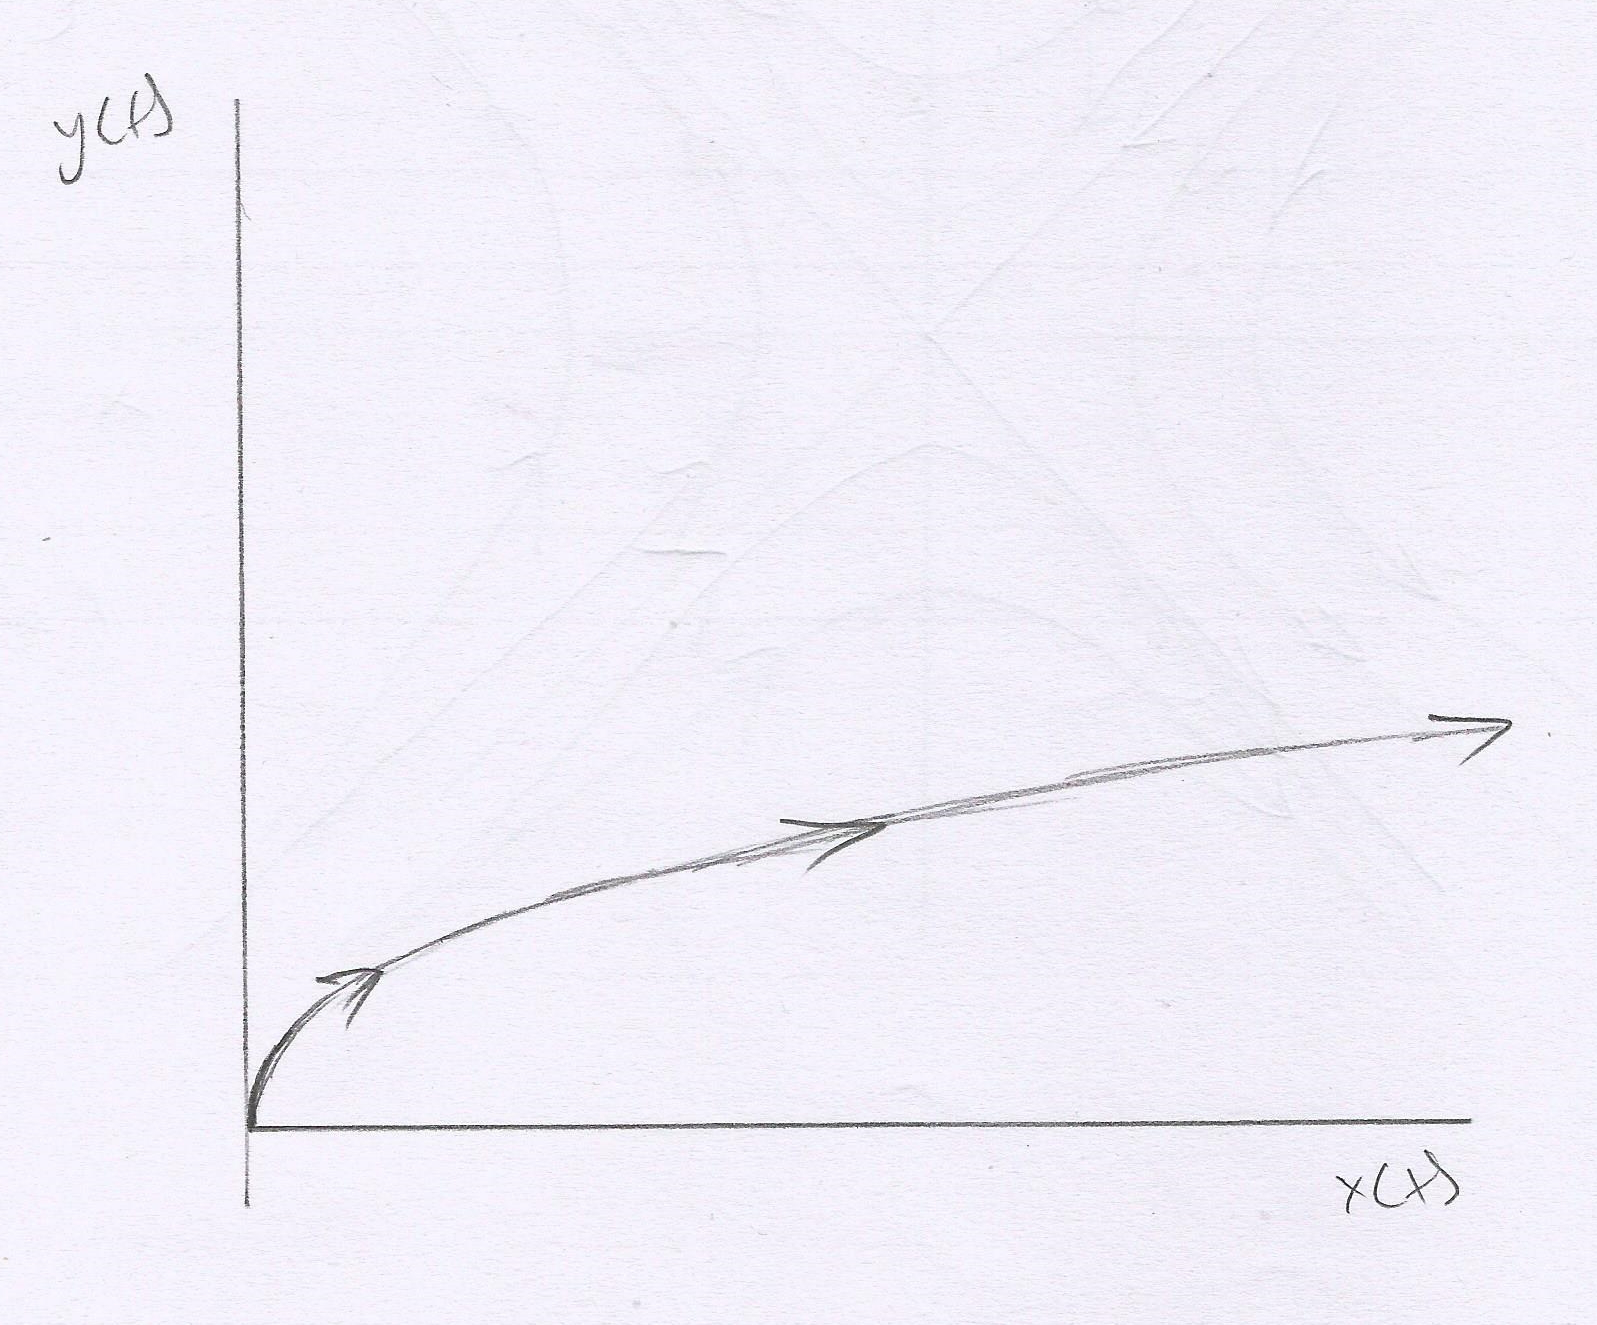
\includegraphics[scale=0.75]{sketch1}
\end{figure}

11. The related phase plane differential equation for the set of autonomous differential equations is:
$$\dv{y}{x} = \frac{x}{y}$$

This is separable, and its general solution is easily found to be $x^2 - y^2 = C$, which form hyperbolae (note $x=0$ or $y=0$ are equilibria). Sketching the family of these trajectories by varying $C$ we have the following:

\begin{figure}[h]
    \centering
    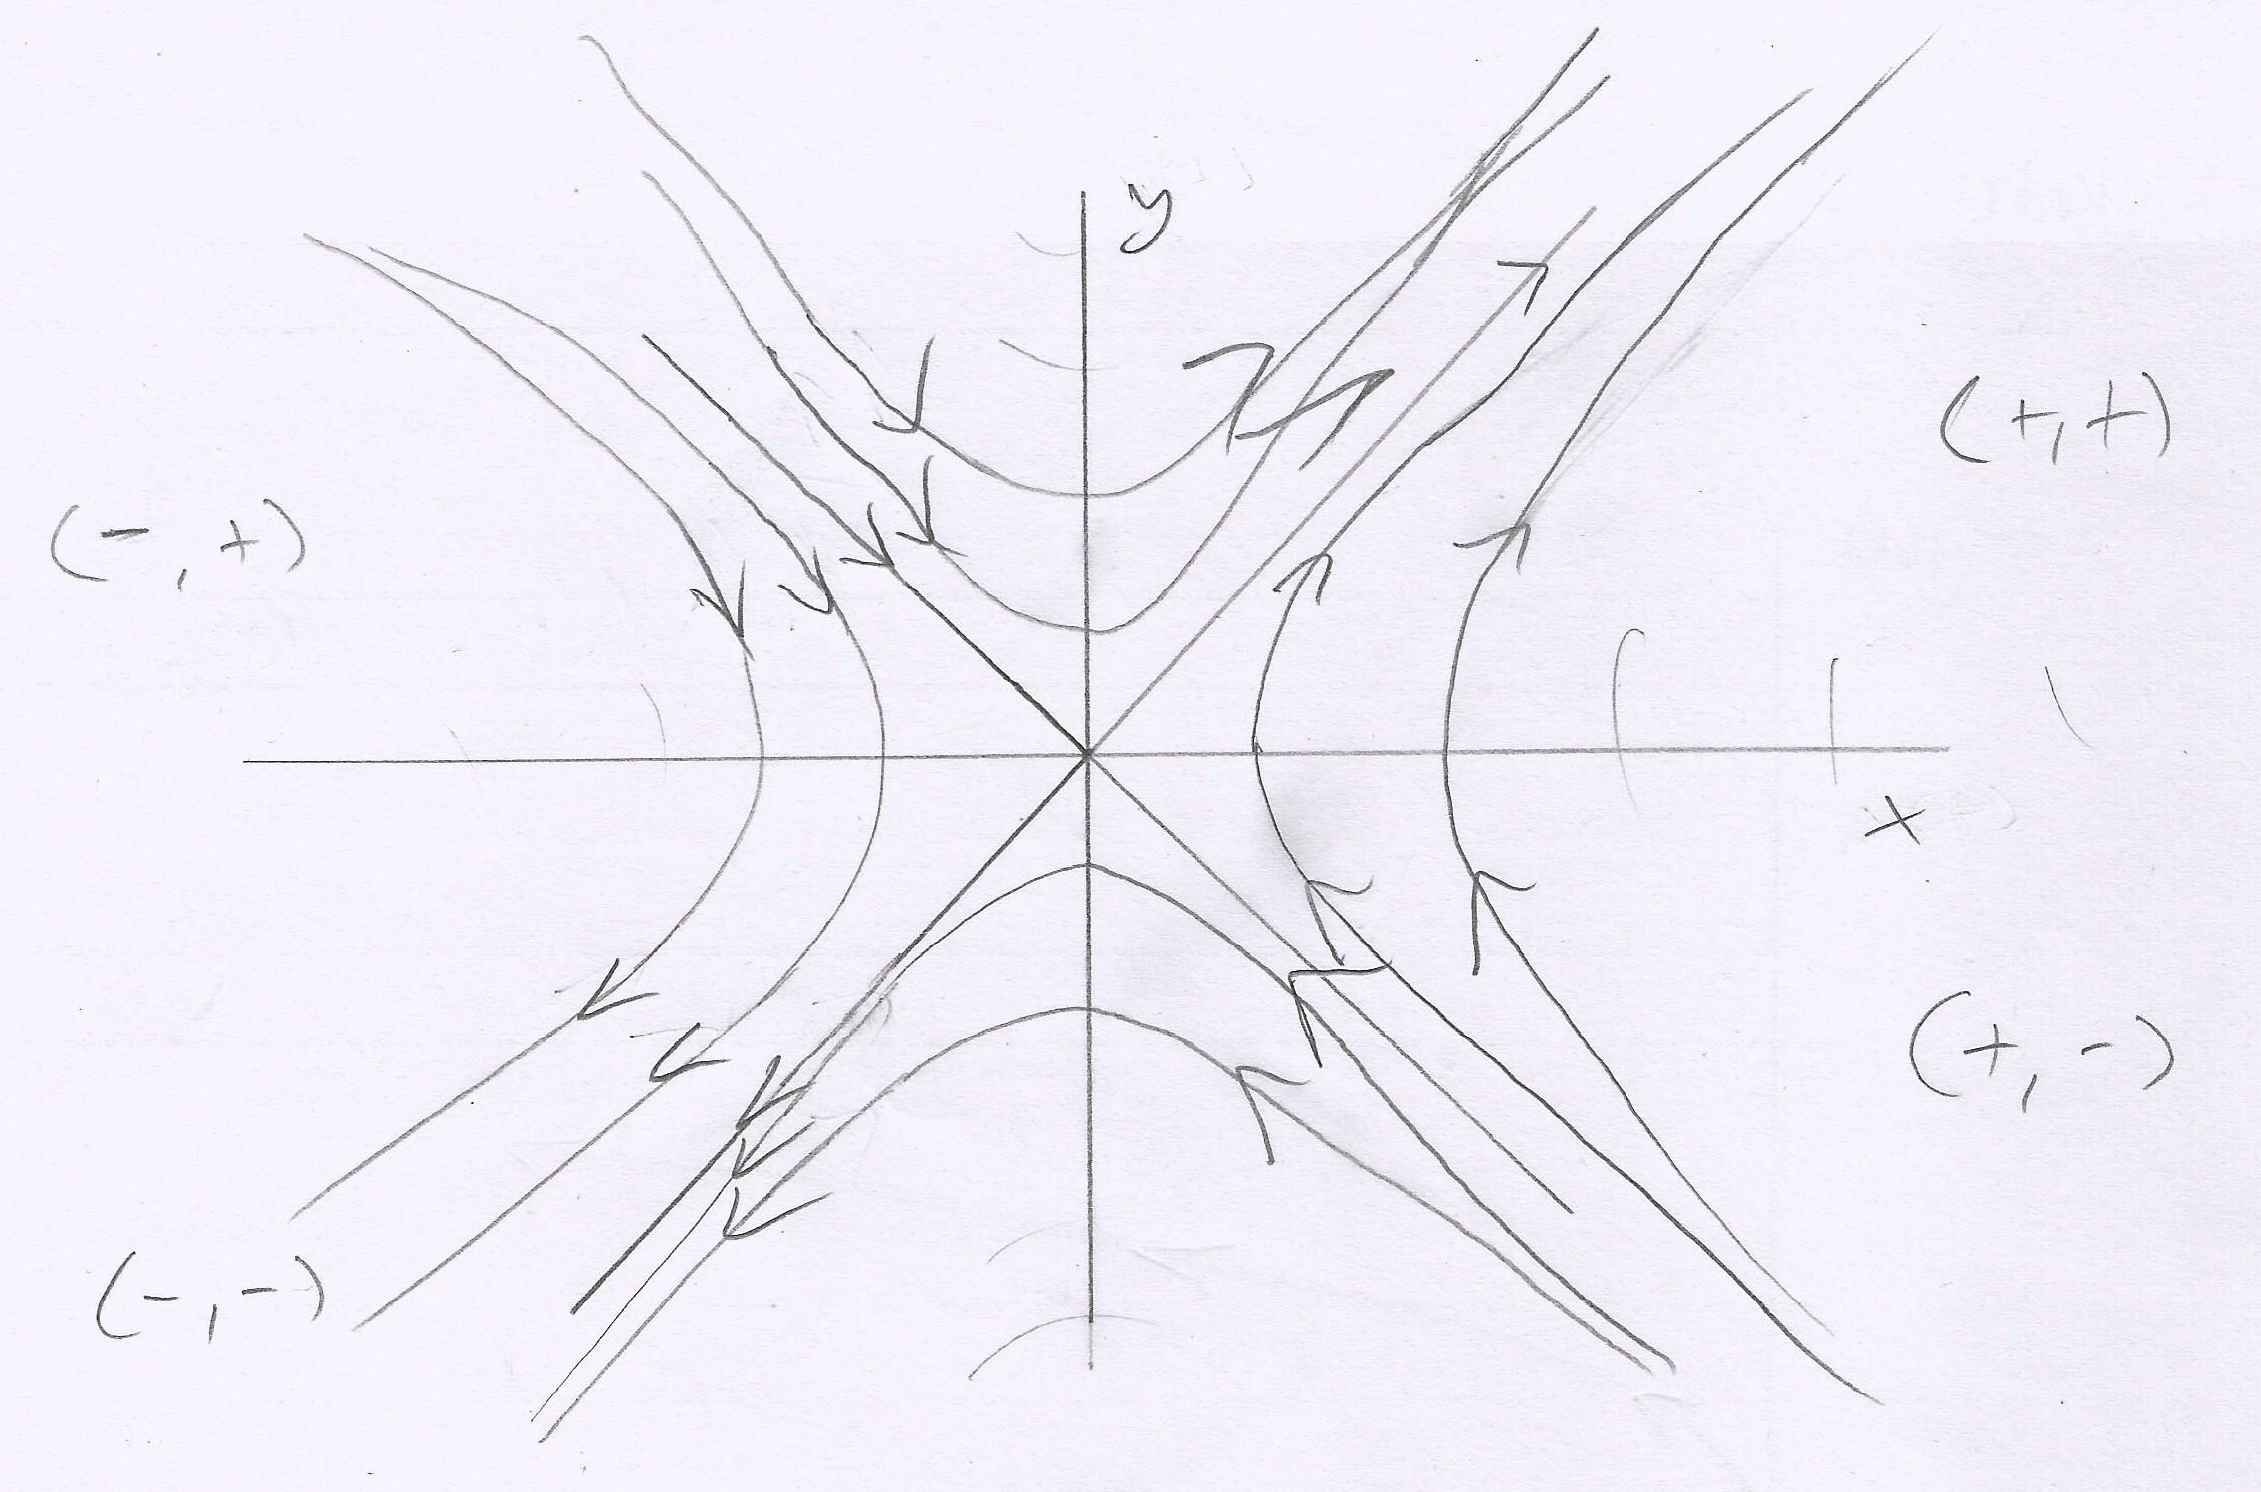
\includegraphics[scale=0.75]{sketch2}
\end{figure}
\end{document}